\chapter{Background}
\label{ch:background}
This chapter will present the necessary background information for this thesis. Here, we define some basic terminology that will be used throughout this thesis.

\section{Defining clones}

\begin{table}[]
\centering
\resizebox{\textwidth}{!}{%
\begin{tabular}{@{}lllll@{}}
\toprule
\textbf{Symbol} & \textbf{Meaning} & \textbf{Description} & \textbf{Contents} & \textbf{Properties} \\ \midrule
\rowcolor[HTML]{EFEFEF}
S & Clone class collection & \begin{tabular}[c]{@{}l@{}}All clone classes that\\ have been found for a\\ certain software project.\end{tabular} & \begin{tabular}[c]{@{}l@{}}Set of clone\\ classes\end{tabular} & - \\
C & Clone class & \begin{tabular}[c]{@{}l@{}}A set of similar code fragments in\\ different locations.\end{tabular} & \begin{tabular}[c]{@{}l@{}}Set of clone\\ instances\end{tabular} & - \\
\rowcolor[HTML]{EFEFEF}
I & Clone instance & \begin{tabular}[c]{@{}l@{}}A code fragment that appears in\\ multiple locations.\end{tabular} & \begin{tabular}[c]{@{}l@{}}Set of cloned\\ nodes\end{tabular} & \begin{tabular}[c]{@{}l@{}}File (F): The file in which this\\ clone instance is found.\\ Range (R): The range this clone\\ instance spans.\end{tabular} \\
N & Node & \begin{tabular}[c]{@{}l@{}}A statement or declaration in a \\ codebase.\end{tabular} & Set of tokens & \begin{tabular}[c]{@{}l@{}}Range (R): The range this node\\ spans.\end{tabular} \\
R & Range & A part of a source code file. & Set of tokens & \begin{tabular}[c]{@{}l@{}}Begin line/column: The line and\\ column at which the range starts.\\ End line/column: The line and\\ column at which the range end.\end{tabular} \\
\rowcolor[HTML]{EFEFEF}
t & Token & \begin{tabular}[c]{@{}l@{}}Tokens are the basic lexical\\ building blocks of source code. \\ For this study, this is the smallest\\ relevant entity of a program.\end{tabular} & - & \begin{tabular}[c]{@{}l@{}}Range (R): The range this token\\ spans.\\ Category: Identifier, Keyword,\\ Literal, Separator, Operator,\\ Comment or Whitespace\end{tabular} \\ \bottomrule
\end{tabular}%
}
\caption{Clone related terminology and how it maps to the source code.}
\label{tab:clone-terminology}
\end{table}

\subsection{Clone Class}
As code clones are seen as one of the most harmful types of technical debt, they have been studied very extensively. A survey by Roy et al \cite{roy2007survey} states definitions for various important concepts in code clone research. In this survey, he mentions the concept ``clone pair'', which is \textit{a set of two code portions/fragments which are identical or similar to each other}. Furthermore, he defined ``clone class'' as \textit{the union of all clone pairs}. Apart from this, we use the definition ``clone instance'', which is a single code portion/fragment that is part of either a clone pair or clone class.

Figure \ref{fig:clonepair} displays an example of a clone pair or clone class. In this case, both cloned fragments, are found in the same class. Each of the cloned fragments can be defined as a ``clone instance''.

\begin{figure}[H]
	\centering
	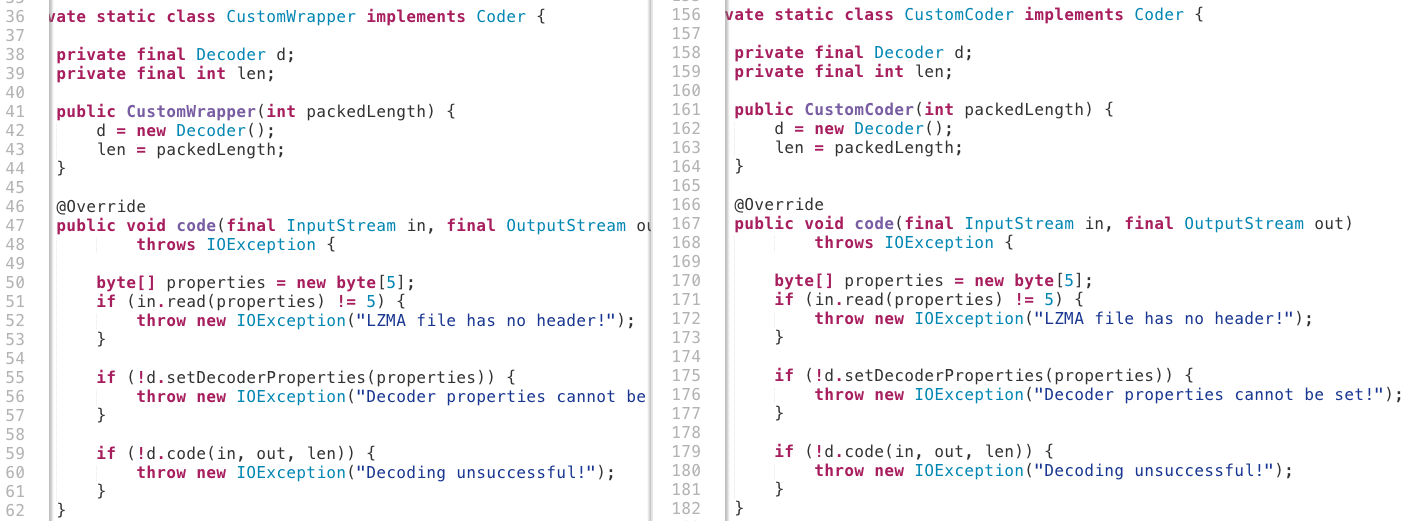
\includegraphics[width=1\textwidth]{img/clone-pair}
	\caption{Example of a clone pair, as found in the \href{https://github.com/Widen/valet}{Valet} project.}
	\label{fig:clonepair}
\end{figure}

Figure \ref{fig:cloneclass} displays a clone class with three clone instances.

\begin{figure}[H]
	\centering
	\includegraphics[width=0.8\textwidth]{img/clone-class}
	\caption{Example of a clone class, as found in the \href{https://github.com/Widen/valet}{Valet} project.}
	\label{fig:cloneclass}
\end{figure}

\section{Clone Types} \ref{chap:backgroundclonetypes}
Duplication in code is found in many different forms. Most often duplicated code is the result of a programmer reusing previously written code \cite{haefliger2008code, baxter1998clone}. Sometimes this code is then adapted to fit the new context. To reason about these modifications, several clone types have been proposed. These clone types are described in Roy et al \cite{roy2007survey}:
\begin{displayquote}
\textbf{Type I:} Identical code fragments except for variations in whitespace (may be also variations in layout) and comments.\\
\textbf{Type II:} Structurally/syntactically identical fragments except for variations in identifiers, literals, types, layout and comments.\\
\textbf{Type III:} Copied fragments with further modifications. Statements can be changed, added or removed in addition to variations in identifiers, literals, types, layout and comments.\\
\textbf{Type IV:} Two or more code fragments that perform the same computation but implemented through different syntactic variants.
\end{displayquote}
A higher type of clone means that it's harder to detect and refactor. There are many studies that adopt these clone types, analyzing them further and writing detection techniques for them \cite{sajnani2016sourcerercc, kodhai2010detection, van2019novel}.

\subsection{Type 4 clones}
For this study we have chosen not to consider type 4 clones for refactoring, because they are both hard to detect and hard to refactor (how to choose the best alternative for a certain computation could be a thesis in itself). A study by Kodhai et al \cite{kodhai2013method} looks into the distribution of the different types of clones in several open source systems (see table 6 of his study). It becomes apparent that type 4 clones exist way less in source code than all of the other types of clones. For instance, for the J2sdk-swing system he finds 8115 type 1 clones, 8205 type 2 clones, 11209 type 3 clones and only 30 type 4 clones. Because of that, we can conclude that type 4 clones are relatively less relevant to study.

\section{Background on refactoring methods}

\section{Clone Contexts} %I don't really like this chapter.
Code clones can be found anywhere in the code. The most commonly studied type of clone is the method-level clone. Method-level clones are duplicated blocks of code in the body of a method. Many clone detection tools only focus on method-level clones (like CPD\footnote{CPD is part of PMD, a commonly used source code analyzer: \url{https://github.com/pmd/pmd}}, Siamese\footnote{Siamese is an Elasticsearch based clone detector: \url{https://github.com/UCL-CREST/Siamese}}, Sysiphus\footnote{Sisyphus crawls the Java library for existing implementations of parts of a codebase: \url{https://github.com/fruffy/Sisyphus}}). The reason for this is that with method-level clones it's most likely that the clones are harmful, and they are more straight-forward to refactor.

A paper by Lozano et al \cite{lozano2007evaluating} discusses the harmfulness of cloning. In this paper the author argues that 98\% are produced at method-level. However, the paper that is cited to support this claim \cite{bergman2004ethnographic} does not conclude this same information. First of all, the study that is referenced uses a very small dataset (460 copy \& paste instances by 11 participants). Secondly, the group of subject only consists of IBM researchers (selection bias). Thirdly, it only focuses on copy and paste instances, as opposed to other ways clones can creep into the code. Finally, the ``98\%'' is not stated explicitly, but is vaguely derivable from one of the figures (figure 1) in this paper. Because of this, there is no reliable overview of how many clones there are in different contexts.

This thesis will focus on measuring how many clones there are per context. This way we can determine the impact of focusing our search on a specific context, like the analysis of only method-level clones. Our hypothesis is that the 98\% claim is not true (we think this should be far less). We also hypothesize that clones in different contexts than method-level are less likely to be harmful and less straight forward to refactor.

\subsection{Clone refactoring in relationship to its context}
How to refactor clones is highly dependent on their context. Method-level clones can be extracted to a method \cite{kodhai2013method} if all occurrences of the clone reside in the same class. If a method level clone is duplicated among classes in the same inheritance structure, we might need to pull-up a method in the inheritance structure. If instances of a method level clone are not in the same inheritance structure, we might need to either make a static method or create an inheritance structure ourselves. So not only a single instance of a clone has a context, but also the relationship between individual instances in a clone class. This is highly relevant to the way in which the clone has to be refactored.

\section{Code clone harmfulness}
There has been a lot of discussion whether code clones should be considered harmful.

Most papers view clones as harmful regarding program maintainability. \textit{``Clones are problematic for the maintainability of a program, because if the clone is altered at one location to correct an erroneous behaviour, you cannot be sure that this correction is applied to all the cloned code as well. Additionally, the code base size increases unnecessarily and so increases the amount of code to be handled when conducting maintenance work.''} \cite{ostberg2014automatically}

However, the harmfulness of clones depends on a lot of factors. A paper by Kapser et al \cite{kapser2006cloning} describes several patterns of cloning that may not be considered harmful. In this paper Kapser names examples where eliminating clones would compromise other important program qualities. Another study by Jarzabek et al \cite{jarzabek2010clones} categorized ``Essential clones'': clones that are essential because of the solution that is being modelled by the program. Overall, many of the benefits of code clones do not apply to most modern object-oriented programming languages.
